

\documentclass[authoryear,3p,times,preprint,review,fleqn]{elsarticle}

% ------------------------
%    Packages used
% ------------------------

% \usepackage[paper=a4paper,top=1.5cm,left=1.2cm,right=0.8cm,
%     foot=1cm,bottom=1.5cm]{geometry}

\usepackage[utf8]{inputenc}    % utf8 support       %!!!!!!!!!!!!!!!!!!!!
\usepackage[T1]{fontenc} 
\usepackage{amsmath,amssymb, amsthm,mathtools,mathrsfs,stmaryrd,titletoc}


% bibtex 
\usepackage{natbib}
% biblatex
% \usepackage[hyperref=true,natbib=true,backref=true,style=authoryear-comp,giveninits=true,maxbibnames=9,maxcitenames=2,uniquelist=false,sortcites=none,doi=false,url=false,eprint=false,uniquename=false,dashed=false]{biblatex}
% \bibliography{mpm.bib,mpm_SS.bib}


%\usepackage{bm}% bold math
%\usepackage[scaled=0.92]{helvet}  % set Helvetica as the sans-serif font
%\renewcommand{\rmdefault}{ptm}    % set Times as the default text font
% need to install mtpro2
\let\Bbbk\relax
%\usepackage[subscriptcorrection,slantedGreek,nofontinfo,mtphrd]{mtpro2}

\usepackage[retainorgcmds]{IEEEtrantools}
\usepackage[usenames]{color}
\usepackage{tabularx}
\usepackage{booktabs}
\usepackage{psfrag}
%\usepackage{scalerel} % for large angle brackets <>, does not work
%\usepackage{cite}
%\usepackage[authoryear,sort,nonamebreak,sectionbib]{natbib} 
%\usepackage[authoryear,nonamebreak,sectionbib]{natbib} 
\usepackage[font=small,labelfont=md]{caption,subfig}
\usepackage{multirow}
\usepackage[T1]{fontenc} % typing french
%\usepackage{fancyhdr}
%\usepackage[english,hyperpageref]{backref}                         
\usepackage[bookmarks=true,colorlinks=true,linkcolor=blue,citecolor=red,backref=page]{hyperref}
\usepackage{makeidx}       % make index
\usepackage{float}         % make new float environment such as boxes (captioned)
\usepackage{listings}      % insert source code   
%\usepackage{bm}
\usepackage{algorithm}
\usepackage{algorithmicx}
\usepackage{algpseudocode}
%\usepackage[ruled,vlined]{algorithm2e}
%\sloppy
%\usepackage{authblk}
\usepackage{verbatim}
\usepackage{numprint}


% nomenclature and glossaries for XFEM, CDM
\usepackage{nomencl}
\usepackage[acronym]{glossaries}

% the following packages just to improve the latex experience 
%\usepackage{silence} %
\usepackage{silence}
\WarningsOff
\usepackage{siunitx}
\usepackage[norefs,nocites,ignoreunlbld]{refcheck} % warning for unreferred figs/tables/equas
% search in the .log file for unused fig to detect figures not referred to in the text.
\usepackage[activate={true,nocompatibility},final,tracking=true,kerning=true,spacing=true,factor=1100,stretch=10,shrink=10]{microtype}
% activate={true,nocompatibility} - activate protrusion and expansion
% final - enable microtype; use "draft" to disable
% tracking=true, kerning=true, spacing=true - activate these techniques
% factor=1100 - add 10% to the protrusion amount (default is 1000)
% stretch=10, shrink=10 - reduce stretchability/shrinkability (default is 20/20)
%\usepackage{varioref}
\usepackage[capitalise]{cleveref} %Basically, cleveref must be loaded last.
% clever ref: instead of Fig.~\ref{d}, use \cref{d} or \Cref{d}  capitalise -> Figure 1
% \crefrange{eq1}{eq5}
\usepackage[textsize=tiny]{todonotes}
\usepackage{nicefrac} % type inline fractions: \nicefrac{1}{2}
\usepackage{setspace}
\usepackage{lineno}  % write numbers for lines
%\usepackage[mediumspace,mediumqspace,Grey,squaren]{SIunits}
\usepackage{totcount} % to count the total number of references and other things
\usepackage[figure,table]{totalcount}
\usepackage{blkarray, bigstrut} % write complicated matrices with borders, see http://mirror.lagoon.nc/pub/ctan/macros/latex/contrib/blkarray/blkarray.pdf
\usepackage{setspace}
\usepackage{tikz}
\usetikzlibrary{arrows,decorations.pathmorphing,decorations.pathreplacing,backgrounds,positioning,fit,matrix,math,shapes.misc}
\tikzset{cross/.style={cross out, draw=black, minimum size=2*(#1-\pgflinewidth), inner sep=0pt, outer sep=0pt}, cross/.default={1pt}}
\usepackage{wasysym}
\usepackage{gensymb} % for degree symbol

\usepackage{pgfplots}
 \pgfplotsset{compat=newest}
 %% the following commands are needed for some matlab2tikz features
 \usetikzlibrary{plotmarks}
 \usetikzlibrary{arrows.meta}
 \usepgfplotslibrary{patchplots}
 \usepackage{grffile}

%\usepackage{underscore}
\usepackage[english]{babel}

%\makeatletter
\renewcommand\fs@ruled{\def\@fs@cfont{\bfseries}\let\@fs@capt\floatc@ruled
\def\@fs@pre{\hrule height 1.2pt depth0pt \kern2pt}%
%\def\@fs@post{\hrule height1.2pt depth0pt \kern2pt}%
\def\@fs@post{\kern2pt\hrule height 1.2pt depth0pt \kern2pt \relax}%
\def\@fs@mid{\kern2pt\hrule\kern2pt}%
\let\@fs@iftopcapt\iftrue}
\makeatother

% index generation
% see LATEX companion p 354
\newcommand{\bs}{\symbol{'134}}%print backslash
\newcommand{\Com}[1]{\texttt{\bs#1}%
\index{#1@\texttt{\bs#1}}}
\newcommand{\Prog}[1]{\texttt{#1}%
\index{#1@\texttt{#1} program }}

% shortcuts

% inner product <x,y>
\newcommand{\ipn}{\langle \cdot , \cdot \rangle}
\newcommand{\ip}[2]{\langle #1 , #2 \rangle}

% norm ||x||
\newcommand{\normn}{\left|\left| \cdot \right|\right|}
\newcommand{\norm}[1]{\left|\left|#1\right|\right|}
\newcommand{\meas}[1]{\left|#1\right|}

% McAuley brackets <x>
\newcommand{\mcauley}[1]{\langle #1 \rangle}

\newcommand{\x}{~$\times$~}
\newcommand{\fig}{Fig.~}
\newcommand{\eref}[1]{(\ref{eq:#1})}
\newcommand{\sref}[1]{\ref{section:#1}}
\newcommand{\fref}[1]{\ref{fig:#1}}
\newcommand{\tref}[1]{\ref{table:#1}}
%\newcommand{\eref}[1]{Eq.~(\ref{#1})}
%\newcommand{\erefs}[1]{Eqs.~(\ref{#1})}
%\newcommand{\fref}[1]{Fig.~\ref{#1}}
%\newcommand{\frefs}[1]{Figs.~\ref{#1}}
%\newcommand{\tref}[1]{Table~\ref{#1}}
\newcommand{\trefs}[1]{Tables~\ref{#1}}
%\newcommand{\sref}[1]{Section~\ref{#1}}
\newcommand{\srefs}[1]{Sections~\ref{#1}}
\newcommand{\crefs}[1]{Chapters~\ref{#1}}
\newcommand{\aref}[1]{Appendix~\ref{#1}}
\newcommand{\tsty}{\textstyle}
\newcommand{\dsty}{\displaystyle}
\newcommand{\D}{\displaystyle}
\newcommand{\arrow}{~$\rightarrow$~}
\newcommand{\otheta}{\overline \theta}
\newcommand{\mathG}{\mathcal{G}}

\newcommand{\mi}{_\mathrm{m}}
\newcommand{\ma}{_\mathrm{M}}

\newcommand{\Mi}{^\mathrm{m}}
\newcommand{\Ma}{^\mathrm{M}}

\newcommand{\dep}{_\mathrm{d}}
\newcommand{\ind}{_\mathrm{i}}

\newcommand{\di}{\mathrm{d}}

\newcommand{\defi}{\mathrel{\mathop:}=}

% abbreviations

\usepackage{xspace}
\newcommand{\eg}{\textit{e.g.}\xspace}
\newcommand{\ie}{\textit{i.e.},\xspace}
\newcommand{\etc}{\textit{etc.}\@\xspace}
\newcommand{\CF}{\textit{cf.}\,}     % i.e.
\newcommand{\cf}{\textit{cf.}\,}     % i.e.
\newcommand{\ETAL}{et. al.\@\xspace}
\newcommand{\etal}{et. al.\@\xspace}
\newcommand{\cmatrixb}{\left\{ \begin{matrix}}
\newcommand{\cmatrixe}{\end{matrix} \right\}}

% general vector/matrix commands:

\newcommand{\tvm}[1]{\textbf{#1}}
\newcommand{\tvms}[1]{$\boldsymbol{#1}$\ }
\newcommand{\vm}[1]{\mathbf{#1}}
\newcommand{\vms}[1]{\mathbf{#1}}
\newcommand{\bsym}[1]{\boldsymbol{#1}}

% vector/matrix for space coordinates 'x' and 'y'

\newcommand{\vx}{\mathbf{x}}
\newcommand{\vy}{\mathbf{y}}
\newcommand{\ve}[1]{\mathbf{e}_{#1}}
\newcommand{\bx}{\boldsymbol{x}}
\newcommand{\vxI}{\mathbf{x}_{I}}
\newcommand{\vj}[1]{\mathbf{#1}_{j}}
\newcommand{\xI}{x_{I}}
\newcommand{\yI}{y_{I}}
\newcommand{\hvx}{\hat{\mathbf{x}}}
\newcommand{\hx}{\hat{x}}
\newcommand{\hy}{\hat{y}}

\newcommand{\trans}{^\mathrm{T}}
\newcommand{\transi}{^\mathrm{-T}}
\newcommand{\el}{_\mathrm{e}}
\newcommand{\pl}{_\mathrm{p}}

\newcommand{\inte} [1]{\int_\Omega #1 d\Omega}
\newcommand{\intE}[1]{\int_{\Omega_0} #1 d\Omega_0}
\newcommand{\intg}[1]{\int_{\Gamma} #1 d\Gamma}
\newcommand{\intG}[1]{\int_{\Gamma_0} #1 d\Gamma_0}



%\newcommand{\T}{\underline{\vm{T}}}

% Shortcuts for making slides

\newcommand{\fontone}{\bfseries\Large}
\newcommand{\fonttwo}{\bfseries\large}
\newcommand{\fontonesc}{\scshape\Large}
\newcommand{\fonttwosc}{\scshape\large}
\newcommand{\fontthree}{\bfseries}
\newcommand{\bc}{\begin{center}}
\newcommand{\ec}{\end{center}}
\newcommand{\bitem}{\begin{itemize}}
\newcommand{\eitem}{\end{itemize}}

% ************************ MATH TYPE MACROS **************************
\newcommand{\mth}[1]{\mathit{#1}}      % print standard math italics
\newcommand{\boldsym}[1]{\mbox{\boldmath${#1}$}}
\newcommand{\vct}[1]{\boldsym{#1}}     % print vector
\newcommand{\fnc}[1]{\prno{#1}}        % print function i.e. sin ...
\newcommand{\mtx}[1]{\mathbf{#1}}      % print matrix
\newcommand{\msc}[1]{\mathcal{#1}}     % print script
\newcommand{\mss}[1]{\mathsf{#1}}      % print sans sarif
\newcommand{\tns}[1]{\boldsym{#1}}     % print tensor
\newcommand{\dbl}[1]{\mathbb{#1}}      % print sets letters like |R |C, etc...
%\newcommand{\Grad}{\stackrel{\rightharpoonup}{\boldsym{\nabla}}\!\!}
                                       % print gradient operator
\newcommand{\GradL}{\!\!\stackrel{\leftharpoonup}{\boldsym{\nabla}}}
                                       % print gradient operator
\newcommand{\Grad}{\boldsym{\nabla}}
                                       % print gradient operator
\newcommand{\Div}{\Grad\cdot}          % print divergnece operator
\newcommand{\DivL}{\cdot\GradL}        % print divergnece operator

\newcommand{\ljump}{\lbrack \! \lbrack } % print left jump oerator
\newcommand{\rjump}{\rbrack \! \rbrack } % print right jump oerator
                                         % derivative
\newcommand{\jump}[1]{\ljump {#1} \rjump} % jump operator
\newcommand{\derivv}[2]{ \frac{d^2 {#1} }{d {#2}$^2$ } }
\newcommand{\deriv}[2]{ \frac{d {#1} }{d {#2} } }   % partial derivivative
\newcommand{\pderiv}[2]{ \frac{\partial {#1} }{\partial {#2} } }
\newcommand{\testspc}{\mathcal{V}}
\newcommand{\trialspc}{\mathcal{S}}

\newcommand{\volint}[1]{\int_{\Omega}\,{#1}\,dV} % integrals
\newcommand{\bndint}[2]{\int_{#1}\,{#2}\,dS}

\newcommand{\beq}{\begin{equation}}
\newcommand{\eeq}{\end{equation}}
\newcommand{\beqa}{\begin{eqnarray}}
\newcommand{\eeqa}{\end{eqnarray}}

%--My own definitions--

\newcommand{\reals}{{\mathbb R}}
\newcommand{\dof}{\emph{dof}}
\newcommand{\dofs}{\emph{dofs}}
\newcommand{\bfalfi}{\mbox{\boldmath$\alpha$\unboldmath$_i$}}
\newcommand{\bfalfj}{\mbox{\boldmath$\alpha$\unboldmath$_j$}}
\newcommand{\remark}[2]{\vspace{0.1cm}
\noindent {\bf Remark #1:}  {#2}  \vspace{0.1cm}}
\newcommand{\invisible}[1]{}
\newcommand{\bgl}[1]{\mbox{\boldmath$#1$\unboldmath}}
\newcommand{\parti}[2]{\frac{\partial #1}{\partial #2}}

% X-FEM related
\newcommand{\xfemlong}{\textit{eXtended Finite Element Method}\,}     % extend..
\newcommand{\xfem}{\textit{X-FEM}\,}     % x-fem

% ********************** VERBATIM AND IGNORE *************************
\newcommand{\bv}{\begin{verbatim}}
\newcommand{\V}{\verb}                  % EX: \V=-d{#@~}= Expr must
                                        % fit on a line

% ************************ FIGURE COMMANDS ***************************
\newcommand{\testpix}[1]{\fbox{\begin{minipage}[c]{\textwidth}
                      #1 \end{minipage} }}

%\ifpdf
% \newcommand{\putfig}[2]{\includegraphics[scale=#2]{#1.pdf}}
%\else
% \newcommand{\putfig}[2]{\includegraphics[scale=#2]{#1.eps}}
%\fi

\newcommand{\putpstex}[1]{\includegraphics{#1.pstex_t}}
% END FIGURE COMMANDS


 % write numbers for lines
 % comment out for final pdf
%\linenumbers

% cleverref package
\crefname{figure}{Fig.}{Figs.}
\crefname{equation}{Equation}{Equations}

% todonotes on the left margin
\reversemarginpar
%\setlength{\oddsidemargin}{3mm}
%\setlength{\evensidemargin}{-3mm}
%\setlength{\textwidth}{160mm}
%\setlength{\textheight}{220mm}


\renewcommand*{\backref}[1]{}
\renewcommand*{\backrefalt}[4]{[{%
    \ifcase #1 %
          \or Cited on page~#2%
          \else Cited on pages #2%
    \fi%
    }]}
    
% -------------------------
%     Header and footer
% -------------------------

% \pagestyle{fancyplain}
% %\addtolength{\headwidth}{\marginparsep}
% %\addtolength{\headwidth}{\marginparwidth}
% %\renewcommand{\chaptermark}[1]{\markboth{#1}{}}
% \renewcommand{\sectionmark}[1]{\markright{\ #1}}
% \lhead[\fancyplain{}{\bfseries\thepage}]{\fancyplain{}{\bfseries Sec. \thesection}}
% \chead[\fancyplain{}{\bfseries\leftmark}]{\fancyplain{}{\bfseries\rightmark}}
% \rhead[\fancyplain{}] {\fancyplain{}{\bfseries\thepage}} 
% \cfoot{}

%\floatstyle{ruled}
%\newfloat{Fbox}{thp}{lop}[chapter]
%\floatname{Fbox}{Box}
%
%\theoremstyle{remark}                                                                                                       
%\newtheorem{thm}{Theorem}[chapter]                                                                                          
%\newtheorem{rmk}[thm]{Remark}    


%% code listing

\lstloadlanguages{C++,Matlab,Python}
\definecolor{mygreen}{rgb}{0,0.6,0}
\definecolor{darkgray}{rgb}{0.95,0.95,0.95}
\lstset{backgroundcolor=\color{darkgray},
  basicstyle=\color{red}\ttfamily,
  keywordstyle=\color{blue}\bfseries
}

\lstdefinestyle{C++}
{
 basicstyle=\footnotesize, numbers=none, numberstyle=\tiny,%
 showstringspaces=false, language=C++, escapechar=|,frame=tb,
 commentstyle=\color{mygreen}
}


\lstdefinestyle{python}
{
 basicstyle=\scriptsize, numbers=left, numberstyle=\tiny,%
 showstringspaces=false, language=Python, escapechar=|,frame=tb,%
 commentstyle=\color{mygreen},
 morekeywords={inner, Function, TrialFunction, TestFunction, solve, FunctionSpace,VectorFunctionSpace,grad,
 LinearVariationalProblem, LinearVariationalSolver, dx,UnitSquareMesh, lhs, rhs, sym, method, region, dimension,run, solid, ulmpm, tlmpm,linear,cylinder,block,material,fix, group,set_dt,dump,run_time,NULL,initial_velocity_particles,sphere,damage_johnson_cook,shock,johnson_cook,velocity_nodes,x,y,z,T,vx,eos,strength,damage,s11}
}



\lstdefinestyle{commentstyle}{color=\color{green}}

\newcommand{\bfsigma}{\boldsymbol{\sigma}}
\newcommand{\bfepsilon}{\boldsymbol{\epsilon}}
\newcommand{\bfu}{\boldsymbol{u}}
\newcommand{\bfx}{\boldsymbol{x}}
\newcommand{\bfphi}{\boldsymbol{\phi}}
\newcommand{\bftheta}{\boldsymbol{\theta}}
\newcommand{\te}{\text{e}}
\newcommand{\td}{\text{d}}
\newcommand{\tp}{\text{p}}

%-----------------------------------------------------------------------
\newcommand{\tty}[1]{\textnormal{\texttt{#1}}}
\newcommand{\sym}[1]{\textnormal{\textit{#1}}}

\lstloadlanguages{C++,Matlab,Python}
\definecolor{mygreen}{rgb}{0,0.6,0}
\definecolor{darkgray}{rgb}{0.95,0.95,0.95}
\lstset{backgroundcolor=\color{darkgray},
  basicstyle=\color{red}\ttfamily,
  keywordstyle=\color{blue}\bfseries
}

\lstdefinelanguage{Sage}{%
    language     = Python,
   morekeywords={var, latex,  view, show, diff, integral, simplify, simplify_full}
}



\lstdefinestyle{C++}
{
 basicstyle=\footnotesize, numbers=none, numberstyle=\tiny,%
 showstringspaces=false, language=C++, escapechar=|,frame=tb,
 commentstyle=\color{mygreen}
}

\lstdefinestyle{C-numbered}
{
 basicstyle=\footnotesize, numbers=left, numberstyle=\tiny,%
 showstringspaces=false, language=C++, escapechar=|,frame=tb,
 commentstyle=\color{mygreen}
}

\lstdefinestyle{matlab}
{
 basicstyle=\footnotesize, numbers=left, numberstyle=\tiny,%
 showstringspaces=false, language=Matlab, escapechar=|,frame=tb,%
 commentstyle=\color{mygreen},
 morekeywords={cell, ones, repmat, intersect, unique}
}

\lstdefinestyle{latex}
{
 basicstyle=\footnotesize, numbers=left, numberstyle=\tiny,%
 showstringspaces=false, language=[LaTeX]TeX, escapechar=|,frame=tb,%
 commentstyle=\color{mygreen},
 morekeywords={cell, ones, repmat, intersect, unique}
}

\lstnewenvironment{snippet}[1][]
{
 \lstset{style=python, xleftmargin=5mm, gobble=4, #1}
}
{}

\lstnewenvironment{snippetlatex}[1][]
{
 \lstset{style=latex, xleftmargin=5mm, gobble=4, #1,tabsize=3}
}
{}

\lstnewenvironment{code-sage}[1][]%
{
   \noindent
   \minipage{\linewidth}
   \vspace{0.5\baselineskip}
  \lstset{style=Sage, xleftmargin=5mm, gobble=4, #1}
}
{\endminipage}

%%

\newcolumntype{C}{>{\centering\arraybackslash}X}
\newcolumntype{b}{X}
\newcolumntype{s}{>{\hsize=0.5\hsize}X}
\newcolumntype{L}{>{\raggedright\arraybackslash}X} 
\newcolumntype{R}{>{\raggedleft\arraybackslash}X} 

\flushbottom

\definecolor{Sun}{rgb}{0.164,0.126,0.322}
\definecolor{Green}{rgb}{0,0.300,0.300}
\definecolor{Red}{rgb}{0.4,0,0}
\definecolor{Grey}{RGB}{105,105,105}
\definecolor{White}{rgb}{1,1,1}

%\newcommand\Algphase[1]{%
%   \vspace*{-.7\baselineskip}\Statex\hspace*{\dimexpr-\algorithmicindent-2pt\relax}%\rule{\textwidth}{0.4pt}%
%      \Statex\hspace*{-\algorithmicindent}\textbf{#1}%
%      \vspace*{-.7\baselineskip}\Statex\hspace*{\dimexpr-\algorithmicindent-2pt\relax}%\rule{\textwidth}{0.4pt}%
%}

% for blocks in Algorithm
\algblockdefx{Start}{End}[1]{\textbf{#1}}{\textbf{end}}

%without this, xelatex would not work with fontspec
\DeclareTextCommand{\nobreakspace}{T1}{\leavevmode\nobreak\ }

%%% vertical rules in cyan color
%\makeatletter
%\renewcommand{\algocf@Vline}[1]{%     no vskip in between boxes but a strut to separate them, 
%  \strut\par\nointerlineskip% then interblock space stay the same whatever is inside it
%  \algocf@push{\skiprule}%        move to the right before the vertical rule
%  \hbox{\bgroup\color{cyan}\vrule\egroup%
%    \vtop{\algocf@push{\skiptext}%move the right after the rule
%      \vtop{\algocf@addskiptotal #1}\bgroup\color{cyan}\Hlne\egroup}}\vskip\skiphlne% inside the block
%  \algocf@pop{\skiprule}%\algocf@subskiptotal% restore indentation
%  \nointerlineskip}% no vskip after
%
\newcommand{\latex}{\LaTeX\xspace}
\numberwithin{equation}{section}

\graphicspath{{./figures/}} 

\newcommand\Lang[1]{\textsc{#1}}

\theoremstyle{remark}
%\newtheorem{thm}{Theorem}[section]
%\newtheorem{rmk}[thm]{Remark}
\newtheorem{rmk}{Remark}

% total number of references
%1. bibtex

% total number of references
\newtotcounter{citenum}
\def\oldcite{}
\let\oldcite=\bibcite
\def\bibcite{\stepcounter{citenum}\oldcite}



%\journal{Advances in Engineering Software}
%\journal{International Journal for Numerical Method in Engineering}

\begin{document}

\begin{frontmatter}



%\title{Modeling crack propagation of concrete gravity dams with the phase-field regularized cohesive zone model}
\title{\textbf{How to effortlessly write a high quality scientific paper in the field of computational engineering and sciences }}

%\tnotetext[label1]{Dedicate to }

% use optional labels to link authors explicitly to addresses:
% \author[label1,label2]{}
% \address[label1]{}
% \address[label2]{}

\author[1]{Vinh Phu Nguyen\corref{cor1}}
 \ead{phu.nguyen@monash.edu}


\cortext[cor1]{Corresponding Author}

\address[1]{Department of Civil Engineering, Monash University, Clayton 3800, VIC, Australia}


%\pagestyle{fancyplain}
%\pagenumbering{arabic}

\begin{abstract}
Starting with a working good research idea, this paper outlines a process that helps us to have a nearly complete paper when the last analysis task is finished.  The key ideas of this process are: (1) writing should start early in the research project, (2) research and writing are carried out simultaneously, (3) best tools for writing should be used.   Due to our personal preferences, the discussion is confined to \LaTeX\ based typesetting. The process seems working well as it has helped us writing thousands of pages without feeling a paint. We hope it works for you too. 

\end{abstract}

% *********************************************************************************************************

\begin{keyword}
 \LaTeX; scientific writing; .
\end{keyword}


\end{frontmatter}



%%%%%%%%%%%%%%%%%%%%%%%%%%%%%%%
\section{Introduction}

\showthe\textwidth % => width of the pdf, see in log file, is 468 pt. use it in plot.py for great plots.

This brief paper gives guidance in writing a paper about your research. Most of the advice applies equally to writing a thesis. Due to our background in .... I have used, as a model, a typical Materials project: one combining experiment with modeling and computation to explain some aspect of material behaviour.

%%%%%%%%%%%%%%%%%%%%%%%%%%%%%%%
\section{Tools}\label{sec:tools}

It is obvious that using a right tool for any task is half way to success. And writing is no exception. Our tools are the following

\begin{itemize}
\item \LaTeX:  a high-quality free typesetting system; it includes features designed for the production of technical and scientific documentation. It is the de facto standard for the communication and publication of scientific documents;
\item \texttt{BibDesk}:  is an open-source reference management software package for macOS, used to manage bibliographies and references when writing essays and articles. It is primarily a BibTeX front-end for use with \LaTeX;
\item \texttt{Adobe Illustrator}: an industry-standard vector graphics software to create high quality drawings;
\item \texttt{Matplotlib}: is a Python 2D plotting library which produces publication quality figures in a variety of hardcopy formats. It can be used in Python scripts;
\item \texttt{Dropbox}: on-going papers are stored in \texttt{Dropbox} so that we can access them from multiple devices;
\item \texttt{Git}: is a distributed version-control system for tracking changes in source code during software development. 
\end{itemize}

The flowchart is as follows. \LaTeX~ is used to typeset the paper. The references used in the paper are stored in a bib file managed by \texttt{BibDesk}. Sketches used in the paper are drawn using \texttt{Adobe Illustrator} and graphs are created using \texttt{Matplotlib}. Sketches and graphs are saved as pdf files and thus of very high quality.

For collaborative writings, \texttt{Git} and \texttt{Github} are very useful. This is because every co-author of the paper can work on the same paper simultaneously and they can use their own favorite \LaTeX\ editor (which is most often also their own coding editor). This is better than \texttt{Overleaf} at \url{https://www.overleaf.com}. And note that \texttt{Github} allows private repositories.

\cref{snippet_penetration}.

\begin{rmk}
Note that \texttt{Bibdesk} is only available for mac OS. One can use \texttt{Zotero} or \texttt{Mendeley} for Windows and Linux computers. Alternatives to the quite pricey  \texttt{Adobe Illustrator} are \texttt{GIMP} or \texttt{Inkscape}.
\end{rmk}

\begin{rmk}
Without going in to the debate which one is the best editor, we use \texttt{Sublime Text}. This is
 because it can be used for both writing \LaTeX\ documents and coding. Furthermore, it can render equations in real time, see  \cref{fig:sublime-text}, which is quite handy. The ability to 

\begin{figure}[h!]
  \centering 
   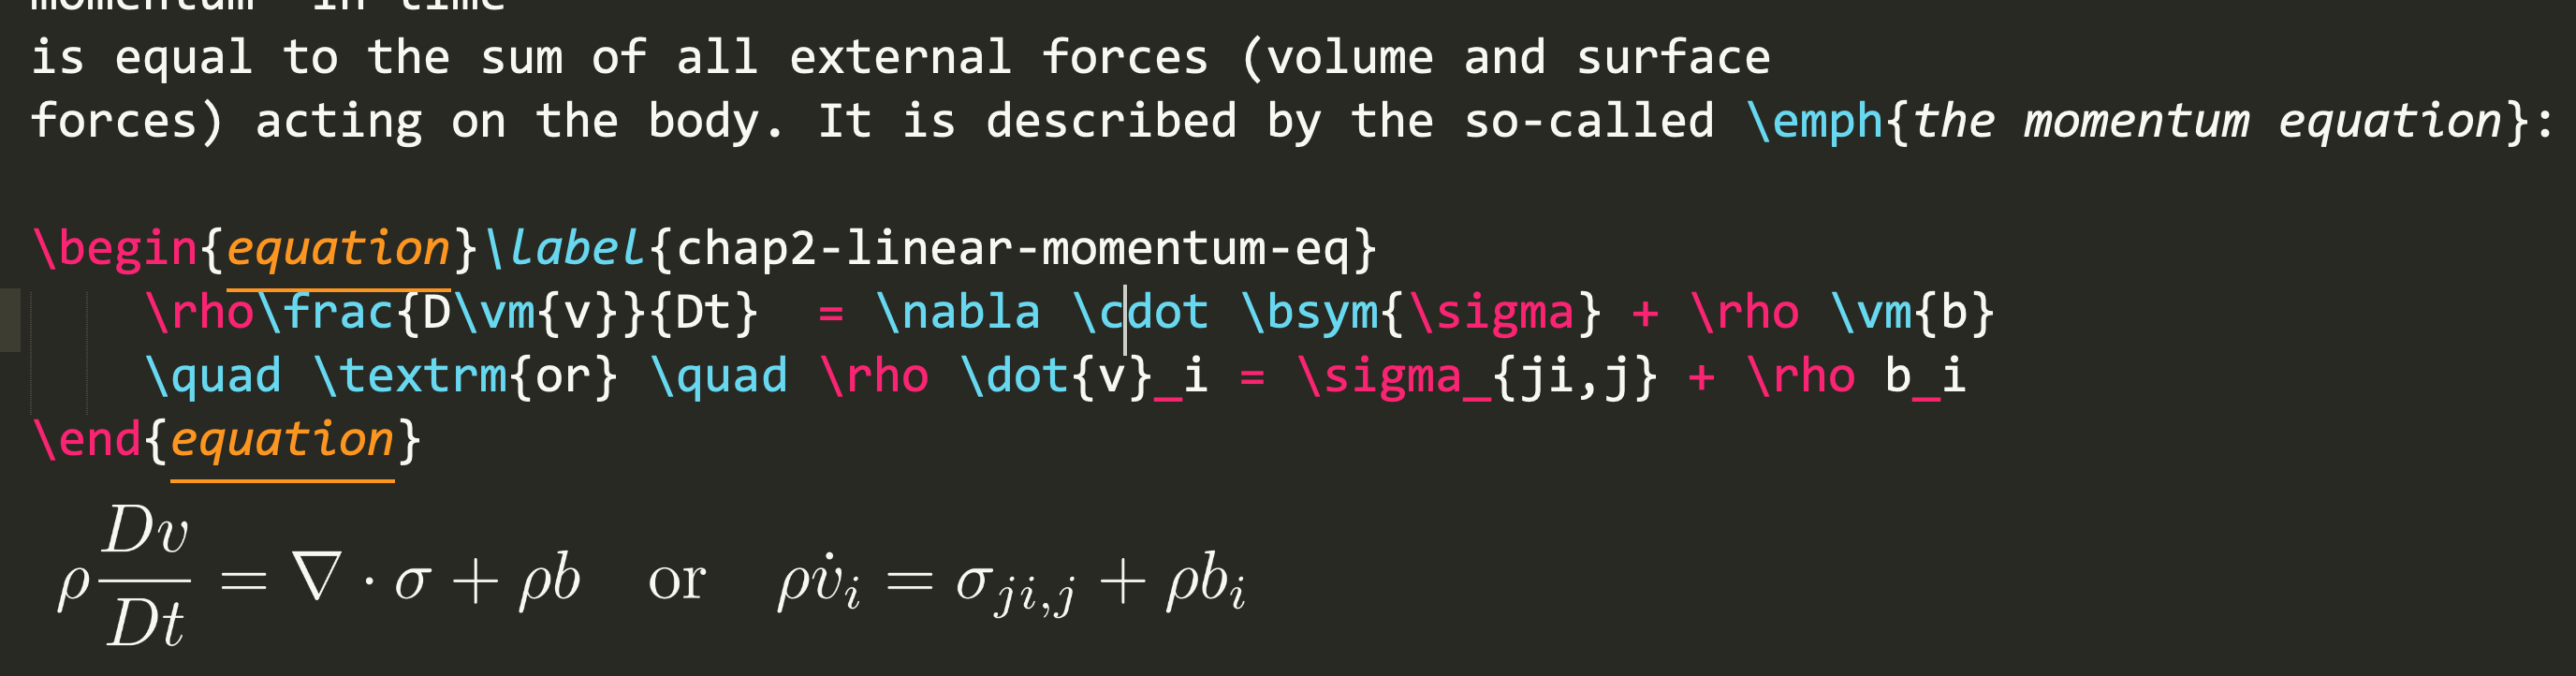
\includegraphics[width=0.65\textwidth]{sublime-text}
   \caption{\texttt{Sublime Text} can render equations in real time.}
\label{fig:sublime-text}
\end{figure}
\end{rmk}


%%%%%%%%%%%%%%%%%%%%%%%%%%%%%%%
\section{Writing tips}\label{sec:writing-tips}

\cref{sec:guidelines}
\cref{sec:writing-process}

\url{https://www.youtube.com/watch?v=VK51E3gHENc}.

%--------------------------------------
\subsection{General guidelines}\label{sec:guidelines}

\begin{enumerate}
\item To inform not to impress;
\item Aims for clarity and readability;
\item Contributions must be clearly stated;
\item Each paragraph conveys only a single idea or message;
\item d 
\item Try to minimize the chances for reviewers to raise issues;
\end{enumerate}

%--------------------------------------
\subsection{Writing process: an iterative process}\label{sec:writing-process}

The first idea is when you have finished your last simulation, the first draft of your full paper is complete. Here by you we mean the co-author of the paper who is in charge of the writing. After that, it is just polishing the paper. The second idea is to not lose motivation due to set backs. That is, if the simulations are not working, don't be upset; let's write something instead. It can be filling Section \textit{Acknowledgments}. Having updated your paper definitely makes us feel good. And that is very important. 


After a research idea has been developed, one should start writing the paper. Obviously, the paper is empty, see \cref{snippet_template} for a \LaTeX\ file for an empty paper.
%---------------------------------------------------------------------------
\begin{figure*}[!h]
  \begin{snippetlatex}[caption={Input file for the plate penetration problem.},label={snippet_template},framerule=1pt,tabsize=3]
    \documentclass[authoryear,3p,times,preprint,review,fleqn]{elsarticle}
    \title{\textbf{}}
    \begin{abstract}
    \end{abstract}
    \section{Introduction}
    \section{Methodology}
    \section{Examples}
    \section*{Acknowledgments}
    \bibliographystyle{abbrvnat} % => just V. P. Nguyen, not Phu Nguyen, ...
    \bibliography{mpm}
  \end{snippetlatex}
\end{figure*}
%---------------------------------------------------------------------------

For the sake of presentation, let's assume that one needs to develop a formulation, implement it in a code, and carry out simulations using this code. Then, one first works on the formulation. When there is some progresses, one can write some key equations in the paper (filling Section \textit{Methodology}). Having the formulations nicely written in a pdf can help you to spot errors. Now that the formulation has been complete, one moves to the implementation. Again, this task should be intertwined  with the writing as well (filling Section \textit{Methodology}). Most often, one starts with a very simple problem to test the code (and the idea). If this example works, one is confident about the idea, he/she can write something on Section \textit{Introduction} while the second simulation is under way. If this example is important, she can write about it in Section \textit{Examples}. If she is lucky, the result of this second simulation is very good. She can now fill  Sections \textit{Introduction} and  \textit{Abstract} while working on the third simulation.

If you feel stuck at writing any parts of the paper, feel free to do something else because keep focusing on the writing does not always help. Most often ideas come when you are in a diffuse mode, a concept proposed in \cite{Oakley:2018a}. For example, while playing with your kids on a playground, the idea for writing a good abstract usually comes. Jotting down the idea on a phone and you're done with this part of the paper.

While working on this paper, we read the literature (we always read it anyway). If we find a good paper relevant to our work, put it in \texttt{Bibdesk}, and cite it in the paper with some key sentences about it. Doing so saves us a lot of time by not re-discovering this paper in the future. Note that \texttt{Bibdesk} can link a pdf to a paper. Therefore, we can have a library of papers on top of a bib file. 

%--------------------------------------
\subsection{Some common mistakes}\label{sec:mistakes}

\cref{tab:mistakes}.

%%%%%%%%%%%%%%%%%%%%%%%%%%%%%%%%%%%%%%%%%%%%%%%%%%
\setlength{\fboxsep}{0pt}
\begin{table}[h!]
   \centering
     \setlength\fboxsep{0pt}
\vskip-\topsep%
\smallskip%
%\renewcommand\arraystretch{1.3}
\colorbox{darkgray}{%
   \begin{tabularx}{0.7\textwidth}{ll}
   \toprule
   Don't & Do  \\
  \midrule
  The Table/Figure 2 & Table/Figure 2 \\
  The Equation (2.2) & Equation (2.2) \\
  \bottomrule
 \end{tabularx}%
 }
\caption{Some common mistakes.}
 \label{tab:mistakes}
\end{table}


%%%%%%%%%%%%%%%%%%%%%%%%%%%%%%%
\section{\LaTeX\ tips}\label{sec:latex}

To improve the writing experience, once in while one should update their \LaTeX\ skills. \cref{snippet_latex_packages} provides an updated list of \LaTeX\ packages being used to write our papers.
By setting the option \textit{backref=page} for the package \texttt{hyperref}, there appears `Cited on page \#' at the end of all references. 

Using standard cross-referencing in \LaTeX\ only produces the label number, a name describing the label such as figure, chapter or equation has to be added manually. The cleveref package overcomes this limitation by automatically producing the label name and number:

\begin{verbatim}
\cref{fig:figure1}, instead of Fig.~\ref{fig:figure1}
\cref{eq:equation1}, instead of Eq.~\ref{eq:equation1}
\end{verbatim}

%---------------------------------------------------------------------------
\begin{figure*}[!h]
  \begin{snippetlatex}[caption={Commonly used \LaTeX\ packages.},label={snippet_latex_packages},framerule=1pt,tabsize=3]
    \usepackage{amsmath,amssymb, mathtools,mathrsfs,stmaryrd,titletoc}
    \usepackage{natbib}
    \usepackage[scaled=0.92]{helvet}  % set Helvetica as the sans-serif font
    \renewcommand{\rmdefault}{ptm}    % set Times as the default text font
    \usepackage[retainorgcmds]{IEEEtrantools}
    \usepackage[usenames]{color}
    \usepackage{tabularx}
    \usepackage{booktabs}    
    \usepackage[font=small,labelfont=md]{caption,subfig}
    \usepackage{multirow}
    \usepackage[T1]{fontenc} % typing french                        
    \usepackage[bookmarks=true,colorlinks=true,linkcolor=blue,backref=page]{hyperref}
    \usepackage{float}         % make new float environment such as boxes (captioned)
    \usepackage{listings}      % insert source code   
    \usepackage{algorithm}
    \usepackage{algorithmicx}
    \usepackage{algpseudocode}
    \usepackage[activate={true,nocompatibility},final,tracking=true,
    kerning=true,spacing=true,factor=1100,stretch=10,shrink=10]{microtype}
    \usepackage[capitalise]{cleveref} %Basically, cleveref must be loaded last.

    % cleverref package: just do \cref{label} for figures, tables, equations anything
    % the package will determine the correct prefix be it Fig. or Equation or Listing.
    \crefname{figure}{Fig.}{Figs.}  
    \crefname{equation}{Equation}{Equations}

    \renewcommand*{\backref}[1]{}
    \renewcommand*{\backrefalt}[4]{[{%
        \ifcase #1 %
              \or Cited on page~#2%
              \else Cited on pages #2%
        \fi%
        }]}
  \end{snippetlatex}
\end{figure*}
%---------------------------------------------------------------------------

It is not a requirement that the font used in figures match that of the text. Yet, it would be better if they match. \cref{fig:cold-spray-plot} is such a figure. And the \LaTeX\ code is shown in \cref{snippet_latex_figure}.

%---------------------------------------------------------------------------
\begin{figure*}[!h]
  \begin{snippetlatex}[caption={Input file for the plate penetration problem.},label={snippet_latex_figure},framerule=1pt,tabsize=3]
    \begin{figure}[!ht]
      \centering
      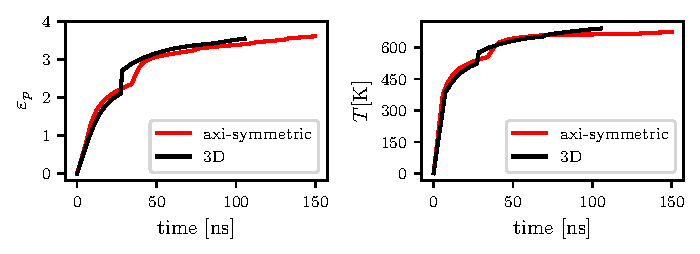
\includegraphics{cold-spray-plots}
      \caption{Cold spraying with a single impact: evolution of plastic strain and temperature.}
      \label{fig:cold-spray-plot}
    \end{figure}
  \end{snippetlatex}
\end{figure*}
%---------------------------------------------------------------------------

\begin{figure}[!ht]
  \centering
  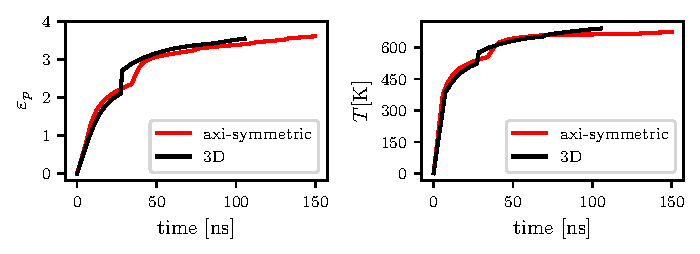
\includegraphics{cold-spray-plots}
  \caption{A figure of which the font matches the text font: 
  evolution of plastic strain $\varepsilon_p$ and temperature time $T=150$.}
  \label{fig:cold-spray-plot}
\end{figure}

%
%%%%%%%%%%%%%%%%%%%%%%%%%%%%%%%
\section*{Acknowledgments}

The first  author gratefully acknowledges the financial support of the Australian Research Council (ARC) Training Centre in Alloy Innovation for Mining Efficiency (IC160100036).
 The second author (V.P. Nguyen) thanks the funding support from the Australian Research Council via DECRA project DE160100577. 

%% The Appendices part is started with the command \appendix;
%% appendix sections are then done as normal sections
%=============================================================================
\begin{appendix}
%=============================================================================
%


\begin{figure*}[!h]
  \begin{snippet}[caption={Input file for the plate penetration problem.},label={snippet_penetration},framerule=1pt,tabsize=3]
    #####################################################
    #               UNITS: GPa, mm, ms                  #
    #####################################################
    # material properties for the steel plate
    E   = 22.4
    nu  = 0.42
    rho = 11.35e-06
    K   = E/(3*(1-2*nu))
    G   = E/(2*(1+nu))
    # Johnson-Cook flow parameters
    sigmay = 12e-3
    B      = 125e-3
    C      = 0
    epsdot0= 1.0
    n      = 1.0
    m      = 1.0
    # Johnson-Cook damage parameters
    d1 = 0.636
    d2 = 1.936
    d3 = -2.969
    d4 = 0
    # problem dimensions
    L, H, W, R, t, d (skip to save space)
    # material props for the projectile 
    m = 20e-3 # kg
    Vol = (4/3)*PI*R*R*R
    density = m/Vol
    Ep = 100
    nup =0
    Gp = Ep/(2*(1+nup))
    Kp = E/(3*(1-2*nup))

    FLIP=0.99
    method(ulmpm, FLIP, linear, FLIP)
    N = 50
    cellsize = L/N
    dimension(3,-2*R-d,2*L,-H,H,-W,W,cellsize)
    # -----------REGIONS ----------------#
    xc = -R-d
    yc = 0 
    zc = 0 
    region(ball,  sphere, xc, yc, zc, R)
    region(plate, block, 0, t, -H, H, -H, H)
    # -----------MATERIALS ----------------#
    eos(eosl, linear, density, Kp)
    eos(eoss, shock,  rho, K, c0, S, Gamma, cv, Tr)
    strength(strengthl,  linear, Gp)
    strength(strengthjc, johnson_cook, G, sigmay, B, n, epsdot0, C, m)
    temperature(tpw, plastic_work, chi, rho, cp)
    damage(damagejc, damage_johnson_cook, d1, d2, d3, d4, epsdot0)
    # Now as EOS, strength, damage and temperature done, build materials
    material(mat1, eosl, strengthl)
    material(mat4, eoss, strengthjc, damagejc, tpw)
    # -----------SOLIDS ----------------#
    ppc1d = 2
    solid(ball,  region, ball,  1,     mat1, cellsize, Tr)
    solid(plate, region, plate, ppc1d, mat4, cellsize, Tr)
    # ----------------- NODE GROUPS --------------------------
    region(region1, block, INF, INF, INF, cellsize/4, INF, INF)
    region(region2, block, INF, INF, H-cellsize/4, INF, INF, INF)

    group(groupn1, nodes, region, region1, solid, plate)
    group(groupn2, nodes, region, region2, solid, plate)

    fix(BC_bot,  velocity_nodes, groupn1, NULL, NULL, NULL)
    fix(BC_top,  velocity_nodes, groupn2, NULL, NULL, NULL)

    #---------- IMPOSE INITIAL CONDITIONS --------------#
    group(gProjectile, particles, region, ball, solid, ball)
    v = 6.58e+3
    fix(v0Ball1, initial_velocity_particles, gProjectile, v, NULL, NULL)

    N_dump = 10
    dump(dump1, all, particle, N_dump, dump_p.*.LAMMPS, x, y, z, damage, s11, vx, T)
    dump(dump2, all, grid, N_dump, dump_g.*.LAMMPS, x, y, z, vx)

    dt_factor(0.5)
    N_log = 10
    set_output(N_log)
    run(150000)
  \end{snippet}
\end{figure*}


\end{appendix}


%%%%%%%%%%%%%%%%%%%%%%%%
\section*{References}


% %%%%%%% BIB files (bibtex)
%\bibliographystyle{plainnat}
\bibliographystyle{abbrvnat} % => just V. P. Nguyen, not Phu Nguyen, ...
%\bibliographystyle{natbib}
\bibliography{writing}

% if biblatex is used
%\printbibliography

\end{document}
